% __BIT_TITLE__
% OrbBits TikZ conventions: see docs/style/tikz.md
\documentclass[tikz,border=6pt]{standalone}
\usepackage{amsmath,amssymb}
\usetikzlibrary{calc,arrows.meta,angles,quotes}

% Project palette (keep colours semantic, not decorative)
\definecolor{orbPrimary}{HTML}{1F5FBF}
\definecolor{orbAccent}{HTML}{E0A100}
\definecolor{orbMuted}{HTML}{7A7A7A}

\begin{document}
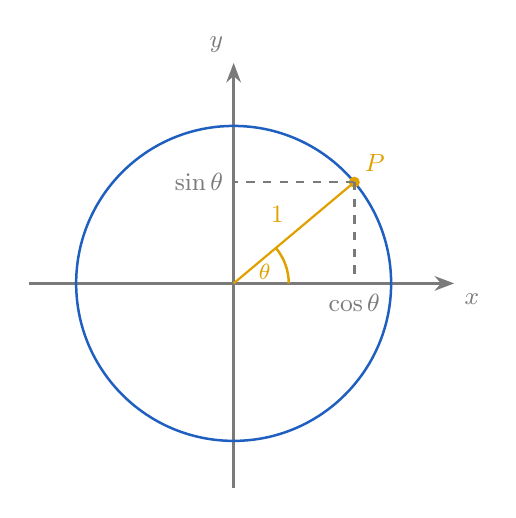
\begin{tikzpicture}[
    >=Stealth,
    line width=0.9pt,
    every node/.style={font=\small},
  ]
  % Axes
  \draw[->,orbMuted] (-2.6,0) -- (2.8,0) node[below right] {$x$};
  \draw[->,orbMuted] (0,-2.6) -- (0,2.8) node[above left] {$y$};

  % Unit circle and a point on it
  \draw[orbPrimary] (0,0) circle (2);
  \coordinate (O) at (0,0);
  \coordinate (P) at (40:2);
  \coordinate (X) at (2,0);
  \draw[orbAccent,thick] (O) -- (P) node[midway,above left] {$1$};
  \fill[orbAccent] (P) circle (2pt) node[above right] {$P$};
  \pic[draw,orbAccent,angle radius=7mm,"$\theta$" {font=\footnotesize}] {angle = X--O--P};
  \draw[dashed,orbMuted] (P) -- (P |- O) node[below] {$\cos\theta$};
  \draw[dashed,orbMuted] (P) -- (P -| O) node[left] {$\sin\theta$};
\end{tikzpicture}
\end{document}
